


\definecolor{dkgreen}{rgb}{0,0.6,0}
\definecolor{gray}{rgb}{0.5,0.5,0.5}
\definecolor{mauve}{rgb}{0.58,0,0.82}
\lstset{frame=tb,
  language=Java,
  aboveskip=3mm,
  belowskip=3mm,
  showstringspaces=false,
  columns=flexible,
  basicstyle={\small\ttfamily},
  numbers=none,
  numberstyle=\tiny\color{gray},
  keywordstyle=\color{blue},
  commentstyle=\color{dkgreen},
  stringstyle=\color{mauve},
  breaklines=true,
  breakatwhitespace=true,
  tabsize=3
}


\section{Kaio Ken}

\subsection{Descripción del problema}
\par{El problema se trata de analizar la cantidad de peleas que debe haber entre un grupo de
guerreros, si en cada pelea hay dos bandos a los que pueden pertenecer, para que todos
peleen con todos y en cada pelea estén en uno de los dos bandos. Matemáticamente lo que
proponemos para resolver en problema es: un conjunto, que se divide en dos una cantidad
finita de veces tal que todos los elementos hallan estado en el conjunto opuesto a todos
los demás elementos en elgun momento.}
\par{Observamos que la cantidad de peleas es logarítmica respecto a la cantidad de guerreros o elementos del conjunto principal: si n es potencia de 2 la cantidad de peleas es $\log(n)$ y si n no es potencia de 2 es $\ceil*{\log_2 n}$. Esto es porque en la primer pelea, si establecemos que $\frac{n}{2}$ elementos pertenecen al bando 1 y $\frac{n}{2}$ elementos pertenecen al bando 2, ya tenemos que cada elemento peleó con la mitad del conjunto original. Podemos observar que resta que cada elemento pelee contra sus compañeros de equipo actual. Por lo que, repetimos el paso anterior para cada conjunto de $\frac{n}{2}$ elementos. Y así en $\log_2 n$ peleas cada guerrero habrá peleado con todos los demás, porque el conjunto de n elementos se “divide” en dos cada vez; decimos “divide” porque los equipos son dos siempre: bando 1 y bando 2, pero uso la expresión para explicar cómo obtenemos el resultado de que todos peleen con todos.}
\par{Debemos notar que si la cantidad de elementos es potencia de 2, la cantidad de peleas es exactamente $\log_2 n$. Pero si n no es potencia de 2, voy a necesitar una pelea más para que todos los elementos completen las peleas, es decir que todos terminen de pelear. Esto sucede porque la cantidad de elementos se encuentra entre dos
potencias de 2 (entre $2^{\floor*{\log_2 n}}$ y $2^{\ceil*{\log_2 n}}$), es decir que con ${\floor*{\log_2 n}}$ no alcanza y ${\ceil*{\log_2 n}}$ es el menor número que seguro logra que todos peleen contra todos.}


\subsection{Pseudocódigo}

\begin{algorithm}
\caption{distribuirGuerreros}
\begin{algorithmic}
  \Function{DistribuirGuerreros}{filas: int, columnas: int, matriz: $Arreglo<Arreglo<int>>$ }
	\State int $i \gets 0$ \Comment $\mathcal{O}(1)$
	\State int j \Comment $\mathcal{O}(1)$
	\State int $cambio \gets 0$ \Comment $\mathcal{O}(1)$
	\State int $equipo \gets 1$ \Comment $\mathcal{O}(1)$
	\State int $x \gets 0$ \Comment $\mathcal{O}(1)$
	\While{$i < filas$} \Comment $\mathcal{O}(filas)$
		\State $cambio \gets pow(2,i)$ \Comment $\mathcal{O}(1)$
		\State $x \gets 0$ \Comment $\mathcal{O}(1)$
		\State $j \gets 0$ \Comment $\mathcal{O}(1)$
		\While{$j < columnas$} \Comment $\mathcal{O}(columnas)$
			\If{$x < cambio$} \Comment $\mathcal{O}(1)$
				\State $matriz[i][j] \gets equipo$ \Comment $\mathcal{O}(1)$
			\Else
				\State $equipo \gets ((equipo +1) mod 2)$ \Comment $\mathcal{O}(1)$
				\State $matriz[i][j] \gets equipo$ \Comment $\mathcal{O}(1)$
				\State $x \gets 0$ \Comment $\mathcal{O}(1)$
			\EndIf
			\State $j++$ \Comment $\mathcal{O}(1)$
			\State $x++$ \Comment $\mathcal{O}(1)$
		\EndWhile
		\State $i++$ \Comment $\mathcal{O}(1)$
	\EndWhile
\EndFunction
\end{algorithmic}
\underline{Complejidad:} $\mathcal{O}(filas*columnas)$\\
\end{algorithm}


\begin{algorithm}
\caption{KaioKen}
\begin{algorithmic}
  \Function{Kaioken}{n: int}
	\State int $filas \gets \ceil*{\log_2 n}$ \Comment $\mathcal{O}(1)$
	\State int m[filas][n] \Comment $\mathcal{O}(1)$
	\State distribuirGuerreros(filas, n, m) \Comment $\mathcal{O}(filas*n) = \mathcal{O}(\ceil*{\log_2 n}*n)$
	\\
	\State int $i \gets 0$ \Comment $\mathcal{O}(1)$
	\State int j \Comment $\mathcal{O}(1)$
	\\
	\State imprimir ~filas \Comment $\mathcal{O}(1)$
	\While{$i < filas$} \Comment $\mathcal{O}(filas) = \mathcal{O}(\ceil*{\log_2 n})$
		\State $j \gets 0$ \Comment $\mathcal{O}(1)$
		\While{$j < n$} \Comment $\mathcal{O}(n)$
			\State imprimir ~$m[i][j]+1$ \Comment $\mathcal{O}(1)$
			\State $j++$ \Comment $\mathcal{O}(1)$
			\If{$j < n$} \Comment $\mathcal{O}(1)$
				\State imprimir ~"~ " \Comment $\mathcal{O}(1)$
			\EndIf
		\EndWhile
		\State $i++$ \Comment $\mathcal{O}(1)$
	\EndWhile
\EndFunction
\end{algorithmic}
\underline{Complejidad:} $\mathcal{O}(\log _{2} n * n)$\\
    \underline{Justificación:} $ \mathcal{O}(\ceil*{\log_2 n}*n)$ + $ \ceil*{\log_2 n} * \mathcal{O}(n)$ = $2*\mathcal{O}(\log _{2} n * n)$ = $\mathcal{O}(\log _{2} n * n)$\\
\end{algorithm}

\newpage
\subsection{Demostración de optimalidad}
Se parte de un grupo de $n$ guerreros y se divide en dos grupos de $n/2$ (si n es par; si no, se divide en un grupo de $\ceil*{n/2}$ y en otro de $\floor*{n/2}$). A su vez, cada uno de estos se partirá a la mitad.
Esto se debe a que para pelear a los n guerreros todos con todos se puede organizar una pelea de $n/2$ contra $n/2$ y luego pelear a cada uno de esos conjuntos todos con todos.
\par{Así, se consigue un árbol exactamente binario porque siempre los grupos se dividen en 2 equipos. Las divisiones en equipos terminan cuando quedan $n$ grupos de 1 guerrero porque en ese caso ya habrán peleado todos con todos los $n$ guerreros, es decir, cuando queda un árbol binario con $n$ hojas. Por otro lado, la altura de este árbol es la cantidad de peleas globales que se necesitó organizar, y sabemos que la altura del árbol es mínima cuando el árbol es balanceado, que de hecho es una propiedad que cumple el árbol resultante de dividir siempre a la mitad. Así, se concluye que esta forma de división resulta en el óptimo de peleas globales, que es igual a $\ceil*{\log_2 n}$.}
\par{Esta es la misma explicación de por qué en mergeSort se divide el arreglo a la mitad.}

\subsection{Cota de complejidad}
\par{Como está detallado en el Algoritmo 3, la complejidad del algoritmo propuesto para KaioKen resulta $\mathcal{O}(\log _{2} n * n)$ y de hecho también es $\mathcal{\theta}(\log _{2} n * n)$}.
\par{Este algoritmo no tiene ni mejor ni peor caso dado que siempre se realiza la misma cantidad de operaciones en función de n. Cabe resaltar que en este problema para un determinado tamaño de entrada no se pueden tener diferentes situaciones y el programa siempre lleva a cabo cada instrucción una cantidad fija de veces que depende del n.}
\par{Como se verá más adelante, esto no es así en el Problema 2, en el que puede haber un mismo tamaño de entrada con situaciones muy distintas y disposiciones de androides totalmente diferentes, dando lugar a un mejor y un peor caso del algoritmo propuesto para resolver ese problema. Como en ese caso la información puede ser distinta para un mismo tamaño de entrada cada instrucción se correrá una cantidad de veces que depende de esa información, dando lugar a mayores y menores tiempos de ejecución para el mismo tamaño de entrada.}

\newpage
\subsection{Experimentación}
Realizamos la medición del tiempo de ejecución de la parte del código que calcula la solución y recolectamos los datos expuestos en la siguiente tabla:

\begin{table}[h!]
\centering
\label{my-label}
\begin{tabular}{cc}
\hline
\multicolumn{1}{|c|}{n (Tamaño de la entrada)} & \multicolumn{1}{c|}{Tiempo promedio (nanosegundos)}                                                                                                                                    \\ \hline
\multicolumn{1}{|c|}{10000}                        & \multicolumn{1}{c|}{1689}                                                                                                                                     \\ \hline
\multicolumn{1}{|c|}{15000}                        & \multicolumn{1}{c|}{1889}                                                                                                                                     \\ \hline
\multicolumn{1}{|c|}{20000}                        & \multicolumn{1}{c|}{3051}                                                                                                                                     \\ \hline
\multicolumn{1}{|c|}{25000}                        & \multicolumn{1}{c|}{3616}                                                                                                                                     \\ \hline
\multicolumn{1}{|c|}{30000}                        & \multicolumn{1}{c|}{3794}                                                                                                                                     \\ \hline
\multicolumn{1}{|c|}{35000}                        & \multicolumn{1}{c|}{5612}                                                                                                                                     \\ \hline
\multicolumn{1}{|c|}{40000}                        & \multicolumn{1}{c|}{5735}                                                                                                                                     \\ \hline
\multicolumn{1}{|c|}{45000}                        & \multicolumn{1}{c|}{6550}                                                                                                                                     \\ \hline
\multicolumn{1}{|c|}{50000}                        & \multicolumn{1}{c|}{5798}                                                                                                                                     \\ \hline
\multicolumn{1}{|c|}{55000}                        & \multicolumn{1}{c|}{9041}                                                                                                                                     \\ \hline
\multicolumn{1}{|c|}{60000}                        & \multicolumn{1}{c|}{8217}                                                                                                                                     \\ \hline
\multicolumn{1}{|c|}{65000}                        & \multicolumn{1}{c|}{9236}                                                                                                                                     \\ \hline
\multicolumn{1}{|c|}{70000}                        & \multicolumn{1}{c|}{8781}                                                                                                                                     \\ \hline
\multicolumn{1}{|c|}{75000}                        & \multicolumn{1}{c|}{8025}                                                                                                                                     \\ \hline
\multicolumn{1}{|c|}{80000}                        & \multicolumn{1}{c|}{8841}                                                                                                                                     \\ \hline
\multicolumn{1}{|c|}{85000}                        & \multicolumn{1}{c|}{12973}                                                                                                                                     \\ \hline
\multicolumn{1}{|c|}{90000}                        & \multicolumn{1}{c|}{16051}                                                                                                                                     \\ \hline
\multicolumn{1}{|c|}{95000}                        & \multicolumn{1}{c|}{17312}                                                                                                                                     \\ \hline
\multicolumn{1}{|c|}{100000}                        & \multicolumn{1}{c|}{18256}                                                                                                                                     \\ \hline

\end{tabular}
\caption{Tabla que muestra los tiempos de ejecución correspondientes a distintos tamaños de entrada.}
\end{table}

\par{El gráfico asociado a este experimento es:}
\begin{figure}[h!]
  \centering
  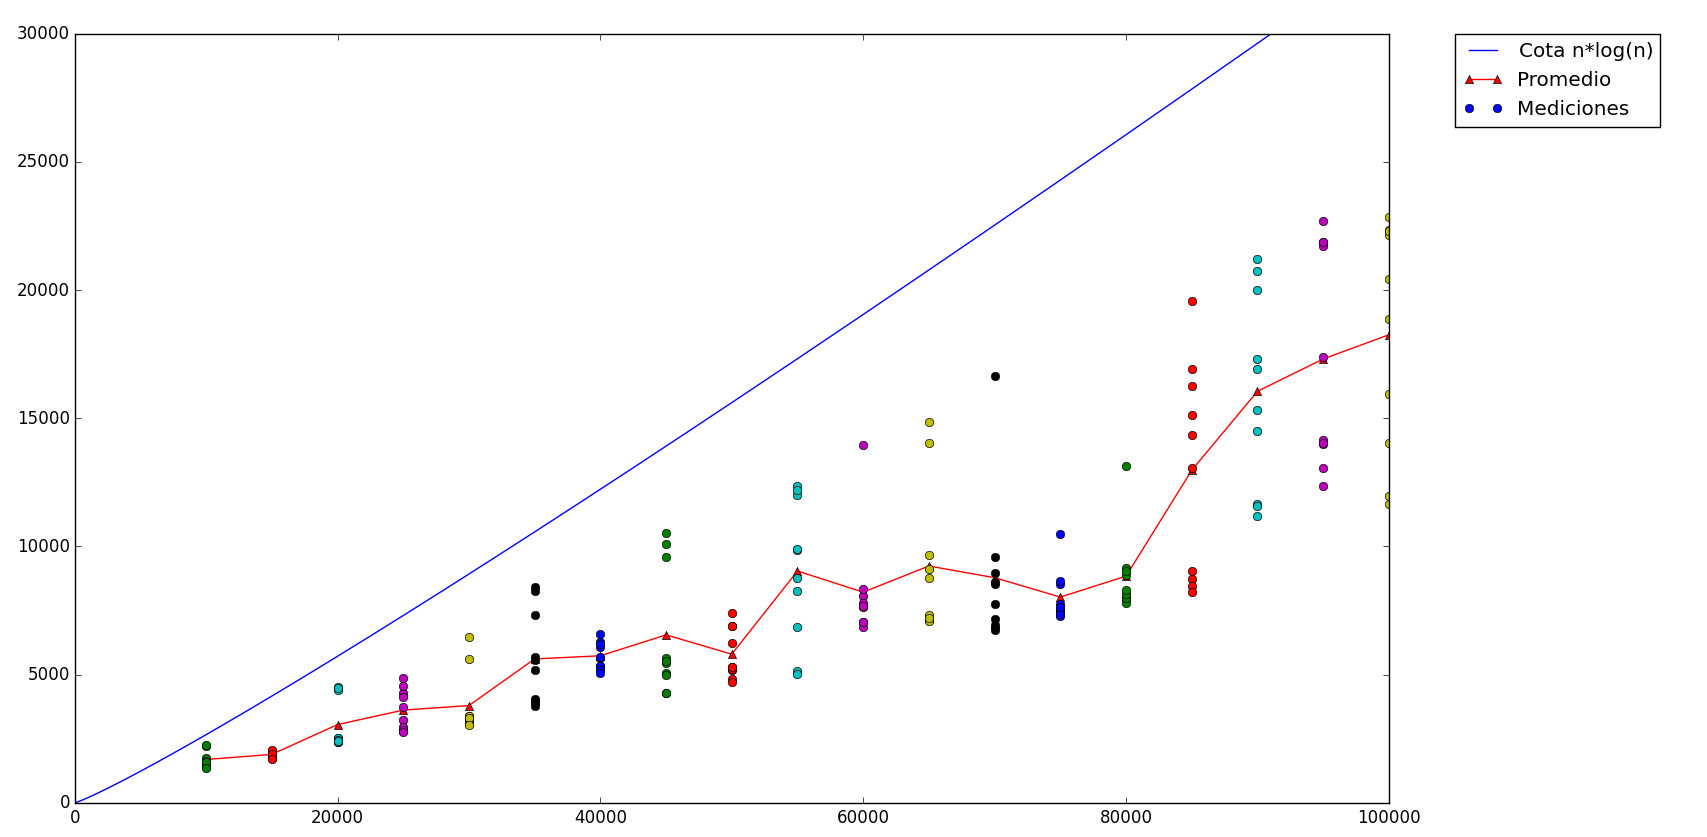
\includegraphics[width=12cm, height=9cm]{tiemposEj1Nuevos}
  \caption{Tiempos de ejecución para distintas entradas. La curva azul es la curva de la complejidad, $n \times \log n$, multiplicada por 0.02, y la roja caso aleatorio.}
\end{figure}

\newpage

\subsection{Apéndice: código de KaioKen}
\begin{lstlisting}
#include <math.h>
#include <stdlib.h>
#include <iostream>
using namespace std;

void kaioKen(int);

int main(int argc, char* argv[]){
	int i;
	cin >> i;
	kaioKen(i);
	return 0;
}

void kaioKen(int n){
	int filas = ceil(log2(n));
	int equipo = 1;
	int cambio = 0;
	int x = 0;
	int m [filas][n];

	//Distribuimos los guerreros
	for (int i = 0; i < filas; i++){
		cambio = pow(2,i);
		x = 0;
		for(int j = 0; j < n; j++){
			if(x < cambio){
				m[i][j] = equipo;
			}else{
				equipo = ((equipo +1) % 2);
				m[i][j] = equipo;
				x = 0;
			}
			x++;
		}
	}

	cout << filas << endl;
	for(int i = 0; i < filas; i++){
		for(int j = 0; j < n; j++){
			cout << m[i][j]+1;
			if (j < n) {
				std::cout << " ";
			}
		}
		cout << endl;
	}
}
\end{lstlisting}
